\chapter{Database Modelling}\label{design}

In order for me to design a complete database model for each of the technologies, an initial investigation into the specific dataset values was required discussed in section \ref{datasetvalues}. Once this was complete I followed the same database design process for each indexing solution which is discussed in section \ref{dbdesign}. A discussion on the data modelling process as whole, for each database system, can be found in section \ref{designdiscussion}

\section{Cleansing the data}\label{datasetvalues}

The EMAGE data which was supplied was made up of 4 tab separated files. Each file contained information pertaining a certain aspect of the dataset; Annotations, Publications, Submissions and Results.

\begin{itemize}
\item \textbf{Annotations} - Data such as the EMAPA structure ID, the EMAPA structure term, the Theiler Stage, the EMAGE structure ID and the strength in which the each gene was detected.

\item \textbf{Publications} - Data regarding all authored publications for the EMAGE dataset. Data included the title, author(s), Theiler Stage and EMAGE ID for the genes.

\item \textbf{Submissions} - Information on each EMAGE assay. Data such as EMAGE ID, Theiler Stage, probe ID, type of assay (in situ or part of), specimen type and specimen strain.

\item \textbf{Results} - Results from each gene expression. Much of the data in this file was a replicated in the submissions file. Data included Theiler Stage, EMAGE ID, data source, assay type and gene name.
\end{itemize}

On initial review each of the files contained similar, repetitive, meta-data values. Thus creating a level of noise which would not add anything to the project in terms of analysis and evaluation. Therefore I undertook an initial cleansing of the data before implementing the database design.

The cleansing process consisted of loading the data into Open Refine (OR) and manually manipulating the data using the filtering and editing tools the package provides. Using OR allowed me to identify any erroneous rows of data which would affect the integrity of the dataset. In each file there was at most 5 rows of data which were either blank or inconsistent with the convention of the rest of the file. I decided to remove these rows as there inclusion in the file was unnecessary.

Another irregularity found in the \textit{Publications} data file was the characters used in the title and author fields. There were over 600 rows of data which contained a non-ascii character. For example - ten Berge D, Brouwer A, el Bahi S, Guénet JL, Robert B, Meijlink F. These rows would be rejected when importing into the databases as by default I decided to apply a UTF-8 character encoding to each indexing solution. Despite these values only contributing to around 5\% of the file, the issue needed to be addressed. To do this I devised a regular expression which would identify and subsequently remove any of these characters.

Using a software tool such as OR enabled me to manipulate and cleanse the data meaning I would be able to load it successfully into the databases. Despite cleansing the datasets successfully, I identified some potential problematic circumstances. While the identified circumstances may not be as significant using the EMAGE dataset, they may affect other big data sets.

The maximum number of rows uploaded into OR was around 150,000. The EMAGE dataset is relatively small in comparison to large scale data collation, however the volume of data was a factor in my decision to use a software tool in an ETL workflow as opposed to rolling my own scripting solution. It is important when choosing a methodology or tool to enhance the veracity of a dataset that the volume of data is taken into consideration. OR is a Java application that utilises the Java Virtual Machine (JVM) and therefore it is integral to allocate enough memory to handle processing large files and thus avoid Java heap space errors. The OR developers suggest that a typical best practice is ``start with no more than 50\% of your available physical memory, since certain OS's will utilize up to 1 Gig or more of physical RAM." \cite{googref}. While using this software solution was sufficient for the data in this project, should the dataset be of a greater scale, a more robust and resilient system would need to be considered.

As discussed in section \ref{5vs} a major challenge in data collection and manipulation is ensuring the veracity of your data. A leading contributor to this challenge is human error. It is a fact of life that humans are error prone and can often make mistakes, therefore where possible the minimal amount of manual handling of a dataset is key. An example of an issue which can arise from this may be as simple as date formatting changing over time. The data may initially be input in a UK standard date format of DD-MM-YYYY by one person and then stored in a US standard data format of MM-DD-YYYY by another person. A simple example, however one which can have serious repercussions on the validity of a dataset. The cleansing of the EMAGE dataset relied on my knowledge of the data and any obvious flaws such as blank values where a value was required. While the data provided was reliable and generally healthy; a richer more granular dataset may require a more rigorous method of validation. One way to do this would be to implement a software script which takes a subset of the data, defines a format, and restructures the remaining data in the dataset accordingly.

\section{Designing the data models}\label{dbdesign}

In order for me to develop multiple and reliable data models which accurately represent the dataset, I created a database diagram for each indexing solution. Each diagram effectively illustrates the relationship between the data entities. The order in which I decided to create the database model designs was based upon two main reasons; which hinge upon aiding the reader's comprehension of this thesis. The first reason was based upon my previous experience of using each of the database systems. My previous experience ranged from a competent level to the complete unknown. Secondly, as MySQL is a well known database management system, and is widely used for a number of applications, it is expected that the reader will already have a functioning knowledge of the system. As a result I decided the first data model I would develop would be for the relational database management system, MySQL. The next system I developed was MongoDB, followed by Neo4j and finally Apache Cassandra. Each implementation presented a different challenge all of which will be discussed below.

\subsection{MySQL - data model design}\label{mysqldesign}

As discussed in section \ref{mysql} MySQL is a relational database management system which stores and represents structured data through entity tables and relationships. There are a number of variations in which the design of the MySQL database could be modelled for the EMAGE data. Figure \ref{fig:mysql} is an entity-relationship (ER) diagram which illustrates the implementation of my MySQL normalised database design. Normalisation in database design is a process by which an existing schema is modified to bring its component tables into compliance through a series of progressive normal forms. Resulting in better, faster, stronger searches. It uses fewer entities to scan in comparison with the earlier searches. Data integrity is improved through database normalisation as it splits all the data into individual entities yet builds strong linkages with the related data. The below description provides an overview into each table and its entities.

\begin{itemize}
\item \textbf{AnatomyStructures} : This table contains the EMAPA ID, and the term which refers to the part of the anatomy. It has a:
\begin{itemize}
\item Many to One relationship with the Stages table, as one anatomy structure can have the same stage.
\item Many to One relationship with itself on the ID, as one structure can have many parts.
\end{itemize} 

\item \textbf{Assays} : This table contains the EMAGE ID number, the ID of the probe and the type of assay. It has a:
\begin{itemize}
\item Many to One relationship with the Sources table. While one assay can only have one source, many assays can have the same source.
\end{itemize} 

\item \textbf{Genes} : This table contains the accession number and symbol of each gene. It has a:
\begin{itemize}
\item The Genes table does not reference any other table.
\end{itemize} 

\item \textbf{Publications} : This table contains the accession, title and every author of each assay publication. It has a:
\begin{itemize}
\item Many to One relationship with the Assays table as there can be many publications for one assay.
\end{itemize} 

\item \textbf{Sources} : This table contains the source of the assay.
\begin{itemize}
\item The Sources table does not reference any other table.
\end{itemize} 

\item \textbf{Specimens} :  This table contains the ID, strain and type of each specimen. The type field refers to whether the assay is a section, wholemount, sectioned wholemount or unknown. It has a:
\begin{itemize}
\item One to One relationship with the Assays table as one assay has one specimen.
\item Many to One relationship with the Stages table as many specimens can have the same Stage.
\end{itemize} 

\item \textbf{Stages} : This table contains the theiler stage and number of days post conception (dpc) of each assay, specimen and anatomy. It has a:
\begin{itemize}
\item Many to One relationship with the Assays table as one assay has can have multiple stages.
\end{itemize} 

\item \textbf{TextAnnotations} : This table contains the structure and strength of each assay. It has a:
\begin{itemize}
\item Many to One relationship with the Assays table as one assay can have multiple text annotations.
\item One to Many relationship with the Genes table as multiple text annotations can the same gene.
\item Many to one relationship with the AnatomyStructures table as many text annotations have one structure.
\end{itemize} 

\end{itemize}

\newpage
\begin{figure}[H]\begin{center}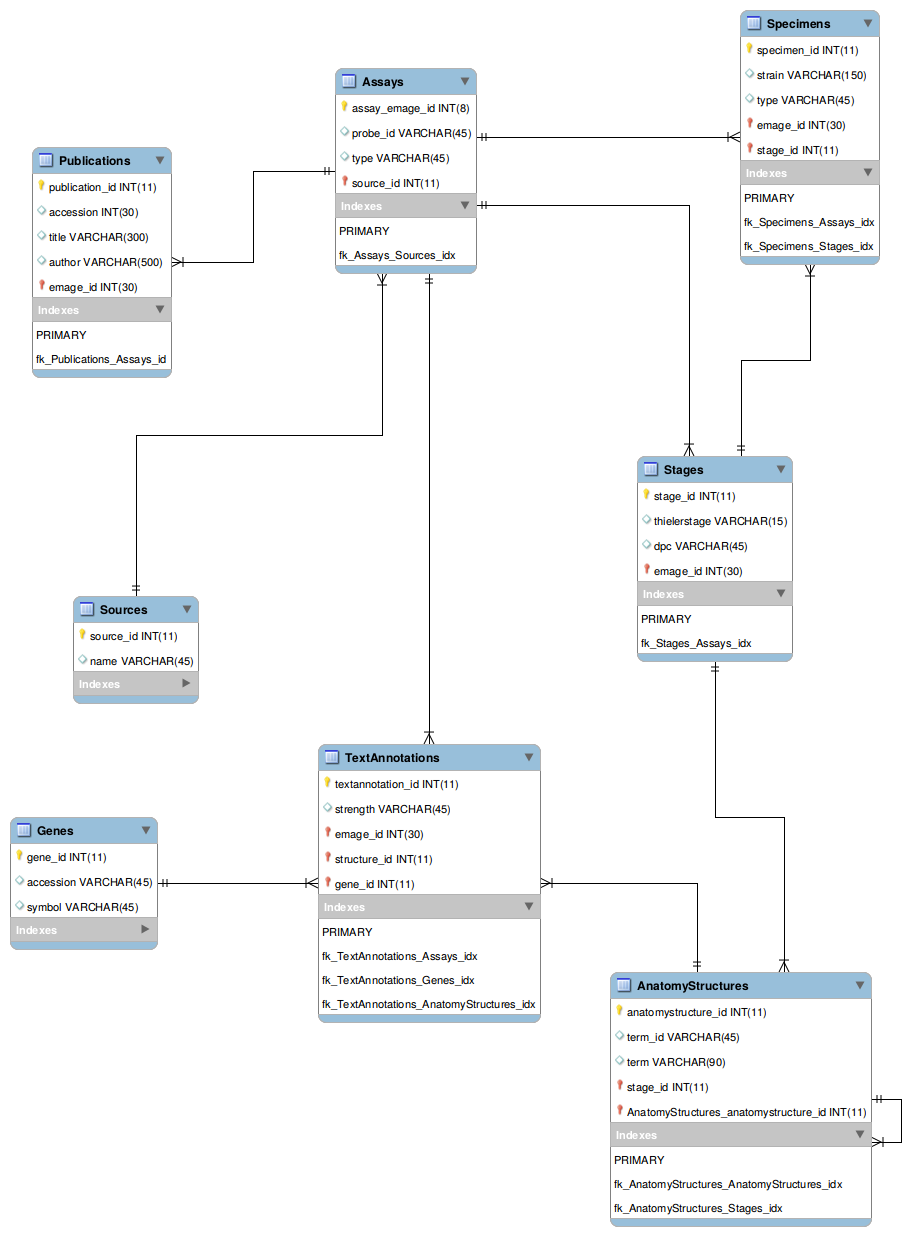
\includegraphics[width=1\linewidth]{images/emage_erd}\caption{MySQL ER table diagram}\label{fig:mysql}\end{center}\end{figure}

\subsection{MongoDB  - data model design}\label{mongodesign}

As discussed in section \ref{mongo}, MongoDB is a homogeneous, schema-less, NoSQL document store database. There are no formal relations between the data, this makes modelling the database more challenging; especially with data which is as closely bound as the EMAGE dataset.

Data in MongoDB sits in \textit{collections}; a grouping of documents which are stored on a database. A collection exists within a single database and is the equivalent of an RDBMS table. Documents within a collection can have different fields and typically all documents in a collection have a similar or related purpose. 

The MongoDB implementation was the second prototype data model I created for this project. I followed the same structural process that I had undertaken for the previous MySQL data model. When creating a MongoDB data model there are a number of factors and considerations which need to be identified before starting the formal implementation. Firstly the biggest decision I deliberated over was how the data should be connected. As there were a few options I decided to explore all of them to fully comprehend the positive and negative aspects of each.

My initial design was based around using multiple collections to store the various aspects of the data. The design followed the MySQL model, with 4 collections; Assays, Text Annotations, Anatomy Structures and Genes. To connect the data and bind the values required an additional manually developed ID field for every document. While this was not a complex task, it was one which I felt was unnecessary and added extra unwanted noise to the data. Using this option would have also incurred more overhead when writing the queries for the database. One would firstly have to connect the data (similar to a RDBMS join) and then include a further query. This can only be done at the application level as opposed to querying directly with the database. Depending on the query and number of collection joins, this may not be overly time consuming. Nevertheless, additional resource is still required. 

After some deliberation, I concluded that the best way to implement the data model was to have all of the data in the one collection. Code snippet \ref{code:mongoload} illustrates an example document in the developed MongoDB data model. The diagram should be read as follows:

\begin{itemize}
\item \textbf{id} : This is the EMAGE id of each assay and is the value which binds all of the data together. The id value has been manually configured to correspond with the EMAGE value.
\item \textbf{specimen} : The specimen value is an array of size 2 which holds data regarding the strain and type of the assay.
\item \textbf{probe id} : This value is the id of the probe accession.
\item \textbf{assay source} : The source in which the assay has been retrieved from.
\item \textbf{assay type} : The type of assay which is being analysed. By type I am referring to whether the assay is \textit{in situ} or otherwise.
\item \textbf{stage} : An array containing the information regarding the stage of the assay; Theiler stage and DPC.
\item \textbf{publication} : An array containing all publication information regarding that specific assay; id, title, author.
\item \textbf{text annotation} : The text annotation array is the grouping of strength, anatomy structure and gene of an assay. An anatomy structure has a term id and the name of the term and a gene has the symbol and id.
\end{itemize}

\newpage
\begin{lstlisting}[language=json,caption=Example MongoDB document., label=code:mongoload]
{
    "_id" : 6,
    "probeID" : "MGI:1334951",
    "source" : "emage",
    "type" : "in situ",
    "specimen" : {
        "strain" : "Swiss Webster",
        "type" : "wholemount"
    },
    "stage" : {
        "dpc" : "7.5 dpc",
        "theilerstage" : 11
    },
    "publication" : [ 
        {
            "publicationID" : 1409588,
            "author" : "Tanaka A, Miyamoto K, Minamino N, Takeda M, Sato B, Matsuo H, Matsumoto K",
            "title" : "Cloning and characterization of an androgen-induced growth factor essential for the androgen-dependent growth of mouse mammary carcinoma cells."
        }
    ],
    "textannotation" : [ 
        {
            "anatomystructure" : {
                "term" : "allantois",
                "structureID" : 16107
            },
            "strength" : "strong",
            "gene" : {
                "name" : "Fgf8",
                "geneID" : "MGI:99604"
            }
        }
    ]
}
\end{lstlisting}
\newpage
\subsection{Neo4j - data model design}\label{neomodel}
Neo4j is a graph orientated, NoSQL database solution. It uses the Property Graph Model methodology of connecting data by nodes and weighted edges. Nodes are the equivalent of a row in a MySQL table and edges are the equivalent of a relation. A full description of Neo4j can be found in section \ref{neo}.

The data model I have constructed for Neo4j, is semantically similar to that of the MySQL implementation. There are 8 classes of nodes, which contain relatively the same data as that of each MySQL table. The main difference between the two systems is how the data is joined. Where MySQL has a foreign key join which connects the nodes; Neo4j has an edge.

As with MongoDB and indeed many NoSQL system, there is no formal way to diagrammatically convey the database ``schema''. To illustrate the Neo4j data model I have created an entity relationship (ER) diagram - figure \ref{fig:neo1} - aiming to convey the look and feel of the graph model. The ER diagram should be translated as: an entity is a node and a join is a relationship. The data within each node is:

\begin{itemize}
\item \textbf{Assay}: These nodes contain data such as EMAGE ID, probe ID and type e.g. ``in situ''. The Assay nodes have 4 self-defining relationships:
\begin{itemize}
\item Assay COMES FROM Source
\item Assay HAS Specimen
\item Assay HAS Stage
\end{itemize}
\item \textbf{Publication}: These nodes contain all publication data which includes title, author and id of each assay publication. The Publication nodes have one relationship:
\begin{itemize}
\item Publication DESCRIBES Assay
\end{itemize}
\item \textbf{Source}: The source nodes have just one field, source name. They define the source of each assay.
\item \textbf{Specimen}: Each assay has a specimen node. These nodes store the specimen strain and specimen type. They have one relationship which is the link between the stage nodes:
\begin{itemize}
\item Specimen HAS Stage
\end{itemize}
\item \textbf{Stage}: The stage nodes contain each Theiler Stage and DPC value.
\item \textbf{Annotation}: These nodes contains information regarding the strength of each annotation. It is the join between the Gene and Anatomy Structure nodes. The annotation nodes have two relationships:
\begin{itemize}
\item Annotation REPORTS Assay
\item Annotation HAS AnatomyStructure
\end{itemize}
\item \textbf{Gene}: These nodes contain all data regarding each gene found. Data such as gene name and gene accession. A Gene node has one relationship:
\begin{itemize}
\item Gene HAS Annotation
\end{itemize}
\item \textbf{AnatomyStructure}: These nodes contain all of the data regarding the respective anatomy structures, such as structure ID and structure term name
\end{itemize}

\begin{figure}[H]\begin{center}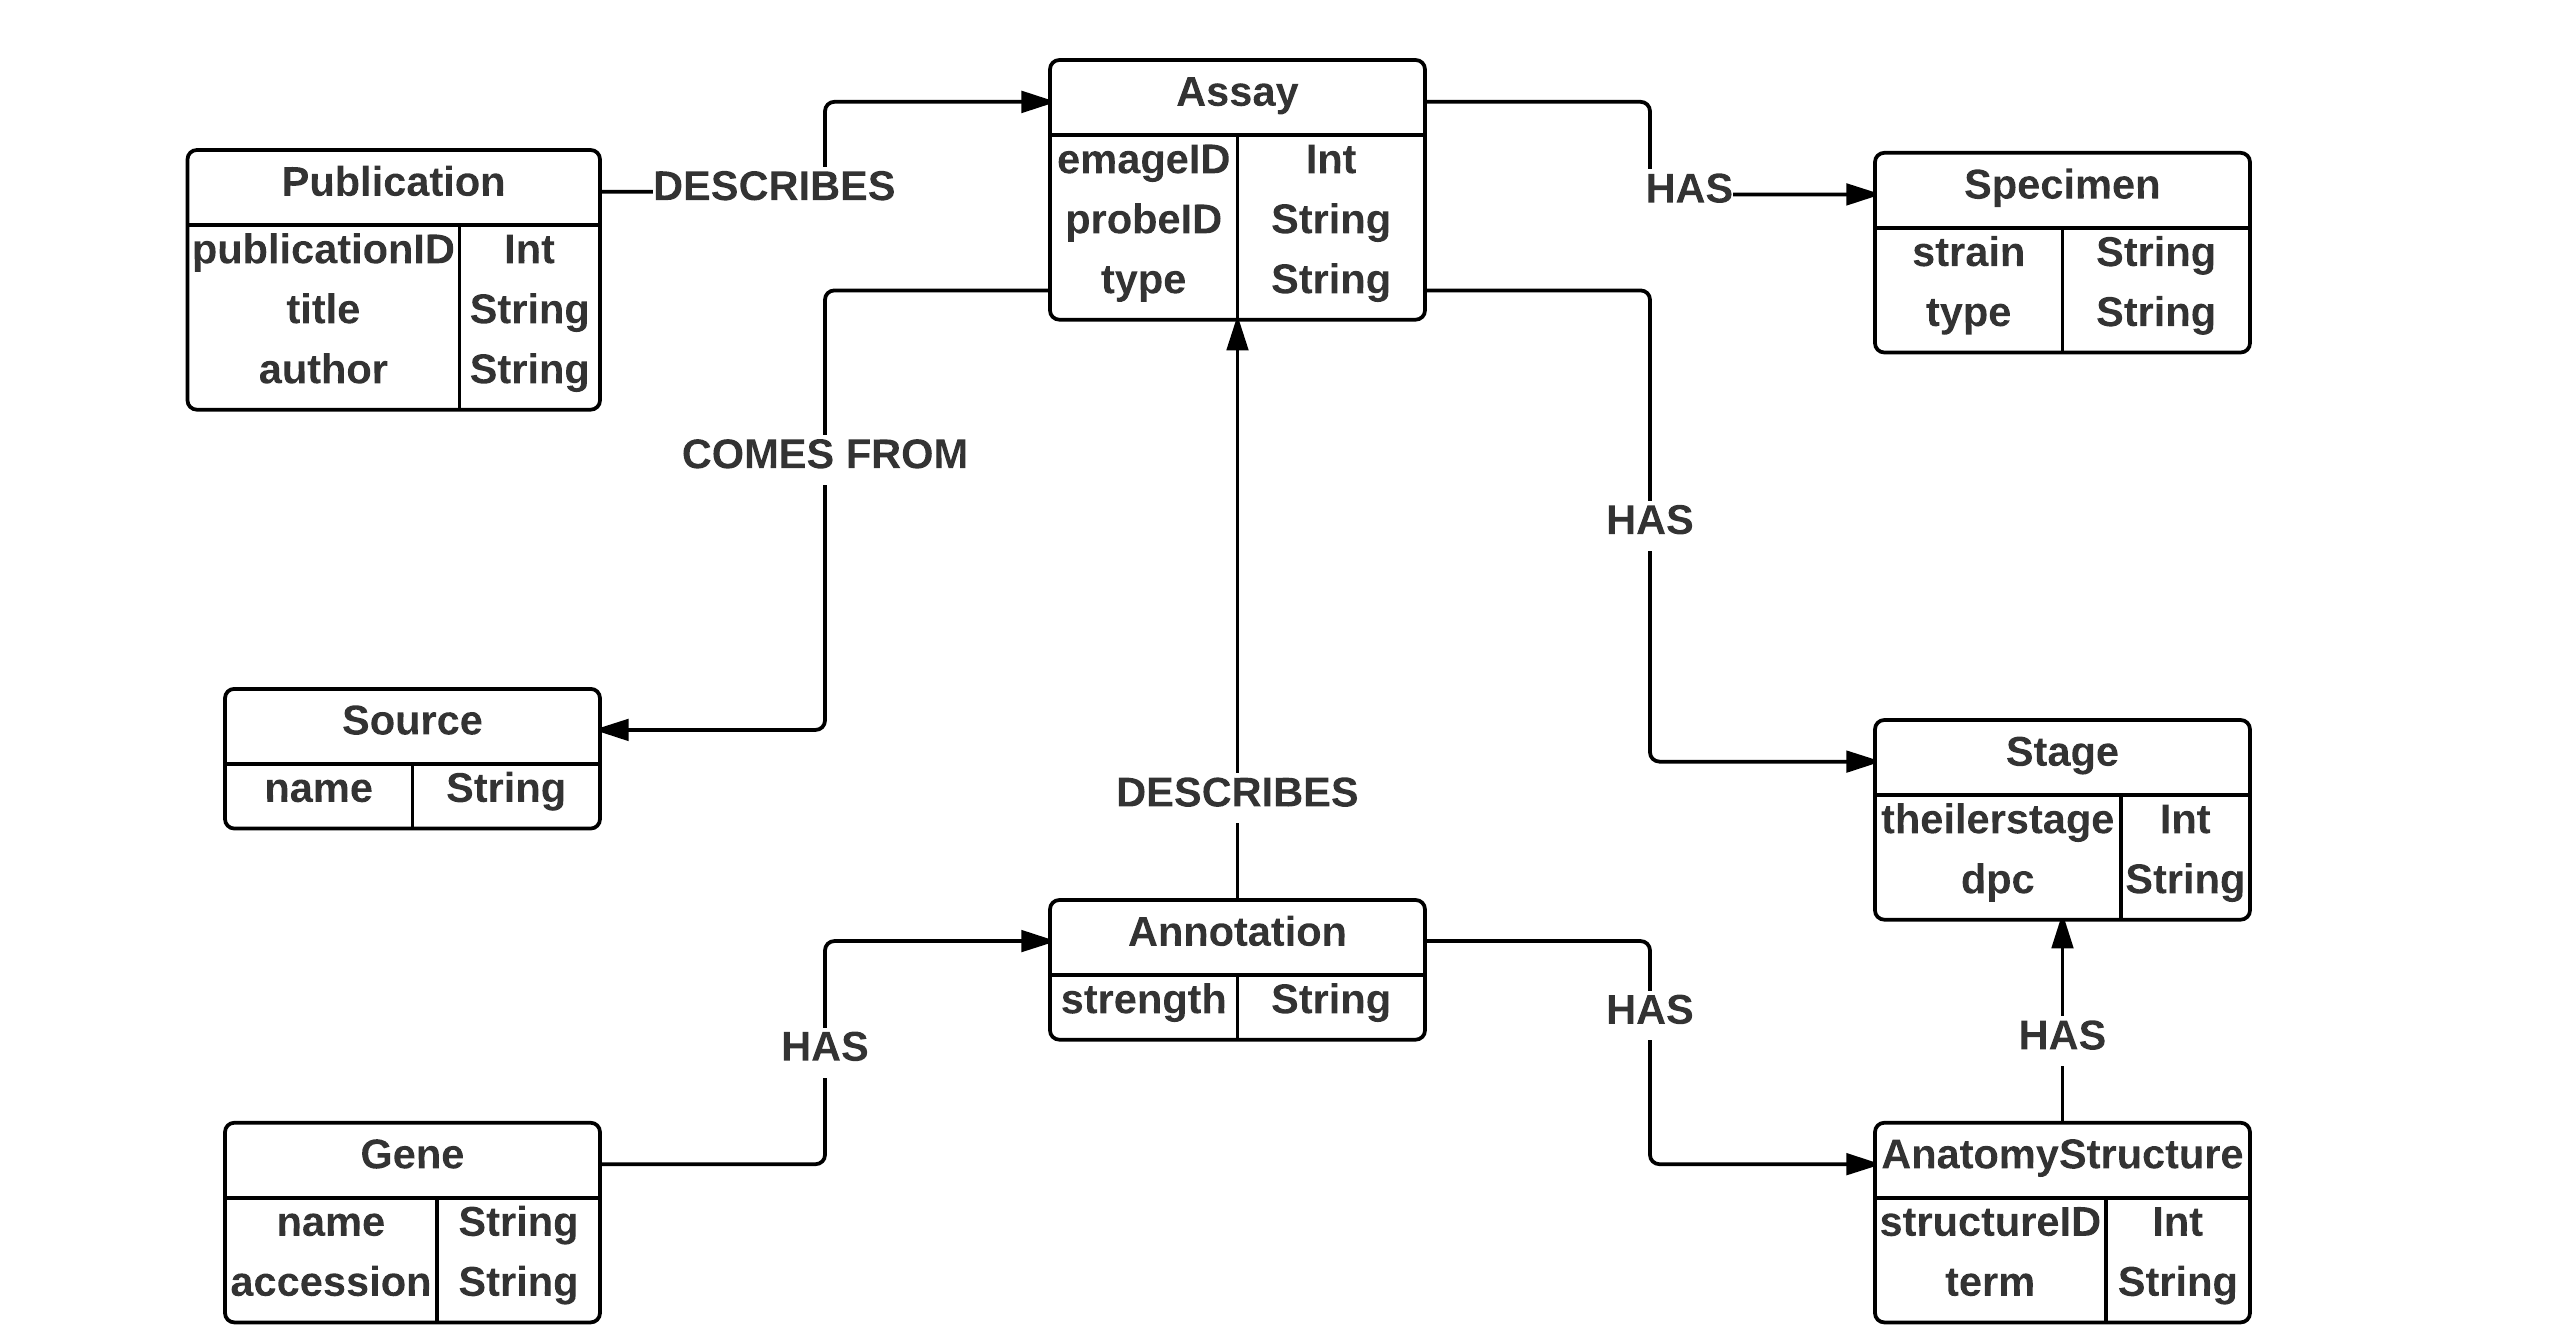
\includegraphics[width=1\linewidth]{images/neo4j_model_er}\caption{Neo4j graph model ER diagram}\label{fig:neo1}\end{center}\end{figure}
\newpage
\subsection{Apache Cassandra  - data model design}
Apache Cassandra is a column based, data management system. A key characteristic of a column based data store is that it is extremely powerful and can be reliably used to keep important data of very large sizes. Despite not being flexible in terms of what constitutes data, it is recognised as being highly functional and performant \cite{cassandra}. With this is mind, normalisation of a dataset is in fact not the optimal way of developing a Cassandra data model. It is proposed that \textit{denormalisation} and data duplication within the data model return the best performing output. This is as a result of Cassandra being optimised to perform a high frequency of writes; this reduces the more costly reads. This is a trade-off which must be taken into consideration when developing the data model \cite{cassandra}.

The Apache Cassandra data model was perhaps the most difficult of all the database system designs to create. This was due to a number of reasons. Firstly, I had no previous experience of using a Cassandra database, and had to learn a completely new style of working. Secondly, as discussed in section \ref{cassandra}, one of the main aspects of Cassandra family columns and tables is that they do not accept joins. This results in tables being created and this aims to satisfy any potential queries which may be imposed on the database. The repercussions of this concept are discussed in section \ref{designdiscussion}.

As with many database systems the optimal way to model a structure is to identify the queries which may be imposed; Apache Cassandra is no different. This can result in multiple tables, containing duplicated data, with either additional or less columns of information. I have modelled the Cassandra data model around the queries outlined in the evaluation strategy of this document (chapter \ref{evaluationstrategy}).

There are 7 tables: Assays, AssayByStage, AssayBySpecimen, Publications, StructureByGene, StructureByStage and TextAnnotations. The naming convention I adopted for the Cassandra data model is based on describing each table by its partition key grouping (for a full description of partition keys and Cassandra concepts, see section \ref{cassandra}). For example, AssayByStage is a table consisting of each Assay partitioned on the Stage value.
\newpage
\section{Discussion - data model design}\label{designdiscussion}
This section provides a general summation of the design process as a whole for each solution. The overall intention of this section, is to provide the reader with an in-depth understanding of the challenges faced and the overall advantages and disadvantages of the data modelling procedures, for each database management system.

The first hurdle one must overcome is to fully comprehend what data they are modelling. Getting to know your dataset, will allow you to develop the optimum system architecture. Having a clear and coherent understanding of how the data is joined and the relationships are formed in your dataset is imperative to a successful outcome. Once an application developer knows what they are developing they can accomplish the how. The design process of a data model can sometimes be overlooked. The two main reasons for this are 1. It is often a challenging process and can be difficult to complete correctly. 2. It can take a long time. Designing the best data model solution for an application can often make or break a project. It is important that the appropriate amount of time is devoted to this process, to ensure that your application sits upon a high performing, durable database system.

The first obstacle I faced was that my knowledge of the EMAP dataset was lacking. I had no prior experience in the biological field and many of the concepts which accompany this dataset took me some time to understand. Therefore being able to logically model a database around an unknown entity was difficult. After discussing the dataset in detail with my supervisors and doing some background research, I was able to surpass this barrier which was slowing my progress in the data modelling phase of the project.

Once the initial hurdle of gaining experience and understanding the theory behind the dataset was overcome, I was able to start physically modelling the systems. In terms of the technical prowess required, depending on field experience, one would be expected to create a data model for each of these systems with relative ease.

With the exception of Cassandra, normalisation and data de-duplication is encouraged for each of the solutions. The objective of database normalisation is to isolate data so that additions, deletions, and modifications of an entity can be made in just one table. In the case of a relational database such as MySQL, this would take the form of splitting one larger table into several smaller tables. An example of this is the Assays table. The Assays table consists of an EMAGE ID, a probe ID and an assay type. The physical data however is made up using the Submissions file (description in section \ref{datasetvalues}). To recap, the submissions file consists of: EMAGE ID, Theiler Stage, Probe ID, the type of assay, the source of the assay, the specimen type and the specimen strain. For the Assays table in the MySQL data model the Theiler Stage, specimen data and the source of the assay have all been split into 3 separate tables. I also split the assay publications, text annotation genes and text annotation structures into separate tables. The tables are joined with either a one-to-one or many-to-one relationship. The MySQL data structure is relatively basic. This was a conscious decision made at the time of design. It can be very easy to complicate and escalate the difficulty of a data model. While normalising a dataset often means creating more tables and thus more relationships, a balance of comprehension vs system performance needs to be found. Implementing the structure in this way makes the information clearer and easier to find for users. It also reduces the need for restructuring the schema, as new types of data are introduced.

A key attribute of MySQL and most relational database systems is its organised rigidity. This requires developers to strictly structure the data which is stored in their applications. Schema alterations are often one of the driving arguments to use a schema-less NoSQL system over a relational database. This was not an issue which I encountered using the EMAGE dataset as it is not dynamic and did not change at all. However, as discussed in section \ref{datasource} the EMAP is ever evolving. There has been many iterations and enhancements made from when the project first began until now. Therefore it is highly likely that, while the current EMAGE structure may be considered the leading source, this will change in the future. The result of this would be that the EMAGE data model would require to be restructured. As this is only a hypothesis we can only speculate as to how the data model would need to be changed. In 2013 a paper published in the Journal of Biomedical Semantics ``EMAP/EMAPA ontology of mouse developmental anatomy: 2013 update'' stated a number of potential future directions of the project. ``Particularly, the ``develops-from'' relationships will be included to support the analysis of differentiation pathways in databases that deal with expression, phenotypic, and disease-related information. Another goal is the inclusion of a set of textual definitions, computable logical definitions that can be used by automated reasoners, and other forms of metadata.'' \cite{biomed}. If we just take the last proposed example of ``other forms of metadata'', in a MySQL data model, depending on the data, this may require an additional table with a join, an index and an ID. The ID would then need to be included into the corresponding table which the data has a relationship. Even for just two or three extra pieces of metadata, the amount of work involved is overly demanding. Comparatively, in a MongoDB data model, should further information become available and require to be included into the database, all that is required is a simple update or insert statement. No restructuring, joining or manipulation of the data model is necessary.

Creating a MongoDB data model is vastly different to that of any of the other solutions in this project. MongoDB imposes a flexible schema, meaning the collections do not enforce a specific structure. This allows one to insert data at their own will without having to conform to a strict schema. It also permits the matching of documents to objects and entities. Because of this, designing the data model was easy. The document structure mirrors that of the EMAGE flat files. Therefore mapping the CSV headings to the Mongo fields was straightforward. As discussed in section \ref{mongodesign} one consideration, specific to the document structure was whether to use embedded documents or multiple collections. The decision to use embedded documents relied heavily on what I was looking to achieve from the project. If I created multiple collections I would have been forced to write cross collection queries, which requires code to be written at the application level. Each of the systems discussed in the project have an API available, mainly Python and Java. While using the API's is perfectly achievable and may be the basis for further research, I focused on what is possible using the command-line interface. 

The most interesting data model for me to create was Neo4j. In terms of the physical structure, I based this mainly on the already created MySQL system. Each table in the MySQL model was mapped as a Neo4j node. The primary key and foreign key relationships in the MySQL system were converted to a relationship in Neo4j. Like relational data models, Neo4j is at its most performant when the nodes are normalised. The clear link between the two systems allowed me to quickly develop a schema for Neo4j. The main aspect of Neo4j which I found to be intuitive and the most useful was the graph model itself. Being able to visualise the nodes as data and and the joins and relationships is clear and extremely easy to follow. There is no complicated joins or key relations to comprehend.

The way in which the Cassandra data model was constructed seemed to me to be rather backwards. Data duplication and de-normalisation was something which was the opposite to what I had been used to for many years using relational databases. Basing the design of the structure on how one is going to query the database was a concept which at first was difficult for me to comprehend. When creating a MySQL system for example, querying the database is often one of the the last considered aspects when data modelling. Flipping the entire process on its head, while refreshing and enjoyable to learn, meant the design stage of the modelling processes was prolonged. This resulted in the overall design of the database being a trial and error exercise. Thus again increasing the time taken to model the system. To the naked eye the design of the tables and the way in which the data is stored could easily be mistaken for a relational MySQL model. The tables are structured similarly and contain many of the same properties. Overall the modelling stage of the Cassandra data model was a steep learning curve. However, as with many processes I often find the best way to learn is to start playing with the software and get used to the concepts. Often failure can be the best way to learn. This was certainly the case with the first stage of the Cassandra data model.





